\documentclass[mathserif]{beamer}

\usepackage{parskip}
\usepackage{amsmath}
\usepackage{amssymb}
\usepackage{graphicx}

\frenchspacing

\logo{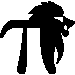
\includegraphics[width=0.075\textwidth]{../Logo}}

\usetheme{Rochester}
\usecolortheme{whale}
%\beamertemplatenavigationsymbolsempty

\AtBeginSection[] {%
	\begin{frame}
		\frametitle{Table of Contents}
		\tableofcontents[currentsection]
	\end{frame}
}

\newenvironment{compactmath}[1][\normalsize]%
	{\begin{minipage}{\textwidth}\vspace{-0.75\baselineskip}#1\begin{equation*}}
	{\end{equation*}\end{minipage}}

\newenvironment{namedframe}[1]%
	{\begin{frame}\frametitle{#1}\framesubtitle{\secname}}
	{\end{frame}}


\title{Summations}
\author{Vincent Macri}
\date{
\includegraphics{../LicenseLogo}\\\copyright{} Vincent Macri, 2017}

\begin{document}
	\frame{\titlepage}
	\section{Basic Sums}
	\begin{frame}
		\frametitle{\secname}
		\framesubtitle{Why we use summation notation}
		\begin{example}
			Add up all of the integers from 1 to 1000. Show your work.
		\end{example}
		This is a fairly easy question, but it takes a long time to do (assuming you aren't using any clever tricks).

		Typing $1 + 2 + 3 + 4 + 5 + \dots + 996 + 997 + 998 + 999 + 1000$ into your calculator will take a long time.

		Surely there is a better way to do this.
	\end{frame}
	\begin{frame}
		\frametitle{\secname}
		\framesubtitle{Summation notation}
		We can use the Greek letter sigma to show a summation:
		\[\sum_{n=1}^{1000}n\]
		This means add up all values of $n$, starting from $n=1$ and going up to $n=1000$.

		Most newer scientific calculators can do summations. If we type the above into our calculator, we will find that:
		\[\sum_{n=1}^{1000}n = 500500\]
		$\therefore$ the answer to our question is 500500.
	\end{frame}
	\section{Advanced Sums}
	\begin{frame}
		\frametitle{\secname}
		\framesubtitle{Another example}
		\begin{example}
			Add up the first 10 positive even numbers.
		\end{example}
		The $n$th positive even number can be written as $2 \times n$.

		We can use this and our calculator to compute our answer:
		\[\sum_{n=1}^{n=10}2n = 110\]
		Since we're only going up to 10, we can check our answer manually:
		\[2 + 4 + 6 + 8 + 10 + 12 + 14 + 16 + 18 + 20 = 110\]
	\end{frame}
	\section{Sum 1 to 100}
	\begin{frame}
		\frametitle{\secname}
		\framesubtitle{The legend of Gauss}
		\begin{example}
			Find the sum of the integers from 1 to 100.
		\end{example}
		Legend has it that the teacher of the famous mathematician Gauss told the class to add up all the numbers from 1 to 100, hoping it would distract them and the teacher would get some time to rest.

		Unfortunately for the teacher, Gauss was very smart and did it in a few minutes.

		Let's look at how.
	\end{frame}
	\begin{frame}
		\frametitle{\secname}
		\framesubtitle{Recognizing patterns}
		If write out the summation twice, but once in reverse, we see an interesting pattern.
		\begin{equation*}
			\begin{array}{lrrrrrrrrrrrrrrrrrrrrr}
				&    &1 &+  &2  &+  &3 &+  \dots &+ &98  &+ &99  &+ &100\\
				&+ &100 &+ &99  &+ &98 &+  \dots &+  &3  &+  &2  &+ &1\\\hline
				&  &101 &+ &101 &+ &101 &+ \dots &+ &101 &+ &101 &+ &101
			\end{array}
		\end{equation*}
		This is $101 \times 100$, which we know is $10100$.

		But we added up the numbers twice, so we need to divide by 2.
		\[10100 \div 2 = 5050 \qquad\qquad \text{\LARGE$\therefore$}\sum_{n=1}^{100}n = 5050\]
	\end{frame}
	\begin{frame}
		\frametitle{\secname}
		\framesubtitle{Making a formula}
		\begin{example}
			Create a formula to find the sum of all the integers from 1 to $n$ for any positive $n$, without using sigma notation.
		\end{example}
		\pause
		We can do something similar as we did in the last example.
		\pause
		\begin{equation*}
			\begin{array}{lrrrrrrrrrrrrrrrrrrrrr}
				&    &1 &+   &2 &+ \dots &+ &n-1 &+ &n\\
				&+   &n &+ &n-1 &+ \dots &+   &2 &+ &1\\\hline
				&  &n+1 &+ &n+1 &+ \dots &+ &n+1 &+ &n+1
			\end{array}
		\end{equation*}
		\pause
		\[\sum_{x=1}^{n}x = \frac{n(n+1)}{2}\]
	\end{frame}
\end{document}
